% !TeX spellcheck = it_IT
\documentclass[10pt,a4paper]{article}

\usepackage[utf8]{inputenc}
\usepackage[T1]{fontenc}	
\usepackage[italian]{babel}
\usepackage{amsmath}
\usepackage{amsfonts}
\usepackage{amssymb}
\usepackage{graphicx}

\usepackage[left=2cm,right=2cm,top=2cm,bottom=2cm]{geometry}
\geometry{a4paper}

\usepackage{booktabs} % for much better looking tables
\usepackage{verbatim}
\usepackage{subfig} % make it possible to include more than one captioned figure/table in a single 

\usepackage{fancyhdr} % This should be set AFTER setting up the page geometry
\pagestyle{fancy} % options: empty , plain , fancy
\renewcommand{\headrulewidth}{0pt} % customise the layout...
\lhead{}\chead{}\rhead{}
\lfoot{}\cfoot{\thepage}\rfoot{}

%%% SECTION TITLE APPEARANCE
\usepackage{sectsty}
%\allsectionsfont{\sffamily\mdseries\upshape} % (See the fntguide.pdf for font help)
% (This matches ConTeXt defaults)

% pacchetti che mi fanno schifo ma uso lo stesso (Bob è scemo, ma anche Ale...)
\usepackage[cdot, thickqspace, squaren]{SIunits}
% il miglior pacchetto che potessi desiderare
\usepackage{float}
% macro che mi piacciono
\def\code#1{\texttt{#1}}


\title{Esercitazione 7: Amplificatore operazionale, usi non lineari}

\author{Gruppo BE \\ Alessandro Candido, Roberto Ribatti}
\date{\today}
\begin{document}
\maketitle

\section{Scopo e strumentazione}

Studiare il funzionamento dell’ OpAmp TL081 in circuiti non lineari, in particolare:
\begin{itemize}
\item un discriminatore,
\item un amplificatore di carica,
\item un trigger di Schmitt,
\item un multivibratore astabile.
\end{itemize}

La strumentazione usata è quella presente sul banco di lavoro, più il suddetto OpAmp e due diodi Zener 1N753A da $\unit{6.2}{\volt}$.

\section{Discriminatore}
Si è montato il circuito in \figurename{~\ref{circuito_discriminatore}} e se ne è studiata la risposta a segnali sinusoidali di frequenza e intensità variabili. In \figurename{~\ref{fig:discriminator}} è mostrato il comportamento ad una frequenza di $\sim \unit{1}{k\hertz}$ ed una tensione di ingresso di $\sim\unit{4}{\volt}$, è visibile l'onda sinusoidale in ingresso e l'onda quadra generata in uscita dall' OpAmp. Poiché l'OpAmp è usato in modalità invertente il comportamento è paragonabile ad un circuito logico NOT.

\begin{figure}[H]
	\begin{minipage}{0.49\textwidth}
		\centering
		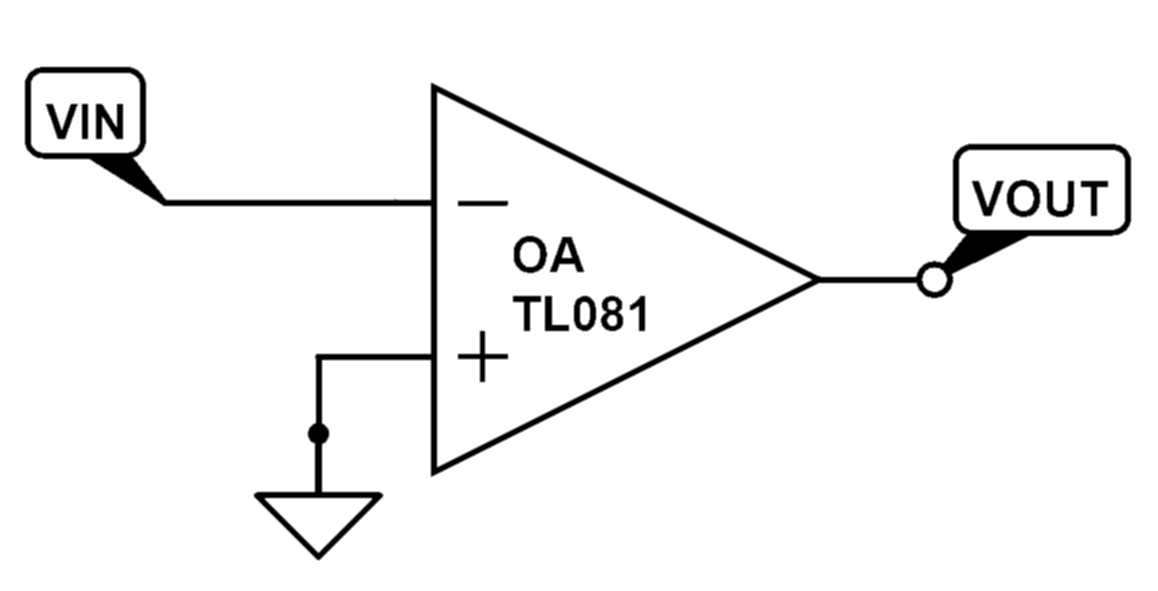
\includegraphics[width=0.7\textwidth]{../circuiti/discriminatore.jpg}
		\caption{Schema del circuito discriminatore}
		\label{circuito_discriminatore}
	\end{minipage}
	\begin{minipage}{0.49\textwidth}
		\centering
		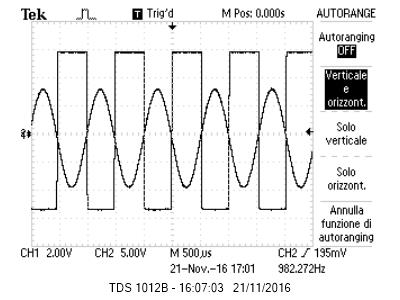
\includegraphics[width=0.9\textwidth]{../oscilloscopio/discriminator.jpg}
		\caption{Risposta del circuito discriminatore}
		\label{fig:discriminator}
	\end{minipage}
\end{figure}

\subsection{Misura della tensione di offset}
Si è proceduto a studiare in maggior dettaglio il punto di zero-crossing e a misurare la tensione di offset $V_{OS}$, ovvero la tensione del segnale sinusoidale $V_{IN}$ nell'istante in cui il segnale in output attraversa lo zero ($V_{OUT}=0$). In \figurename{~\ref{fig:vos}} è visibile il punto di zero crossing e il risultato della misura: $V_{OS} = \unit{150 \pm 5}{\milli\volt}$.

\begin{figure}[H]
	\centering
	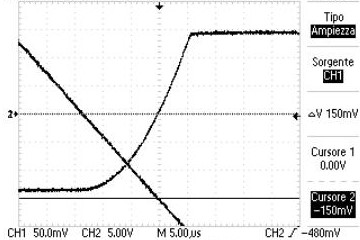
\includegraphics[width=0.45\textwidth]{../oscilloscopio/Vos.jpg}
	\caption{Zoom sul punto di zero-crossing e misura di $V_{OS}$}
	\label{fig:vos}
\end{figure}

\subsection{Conservazione prodotto GBW}
Per elevate frequenze è atteso, per la conservazione del prodotto guadagno-banda che il guadagno dell'OpAmp diminuisca. Per piccoli segnali in ingresso e alte frequenze è possibile quindi che il segnale in output non arrivi a saturazione e sia visibile come un onda sinusoidale.

In \figurename{~\ref{fig:GBW}} è visibile la risposta del circuito ad un segnale di $\sim\unit{100}{k\hertz}$ e un'intensità $V_{IN}= \unit{156 \pm 5}{\milli\volt}$ e come atteso il segnale è sinusoidale.

Si è misurata la risposta a varie frequenze a parità di tensione di input (sempre rimanendo in remime lineare), i dati raccolti sono riportati in appendice in \tablename{~\ref{tab:GBW}}. Si è fittata la conservazione del prodotto banda guadagno $Af_h$, i grafici e i risultati del fit sono riportati di seguito (a e b sono rispettivamente coefficiente angolare e intercetta):

\begin{figure}[H]
	\begin{minipage}{0.28\textwidth}
		\centering
		\begin{tabular}{l}
			$a = \unit{-19.5 \pm 0.7}{\deci\bel / decade}$ \\
			$b = \unit{125 \pm 4}{\deci \bel}$ \\
			$\chi^2 / ndof = 1.9/3$\\
			$corr(a,b) = -0.9987$\\
			$Af_h = \unit{2.57+/-0.16}{\mega\hertz}$
		\end{tabular}
	\end{minipage}
	\begin{minipage}{0.75\textwidth}
		\centering
		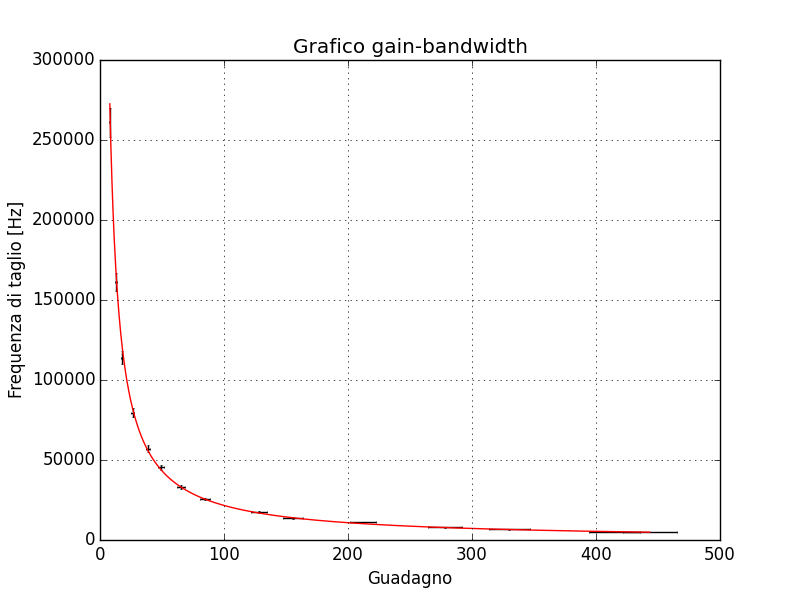
\includegraphics[width=0.95\textwidth]{../grafici/fit_gain_bandwidth.pdf}
		\caption{Dati e fit della conservazione del GBW}
		\label{}
	\end{minipage}
\end{figure}

\begin{figure}[H]
	\begin{minipage}{0.49\textwidth}
	\centering
	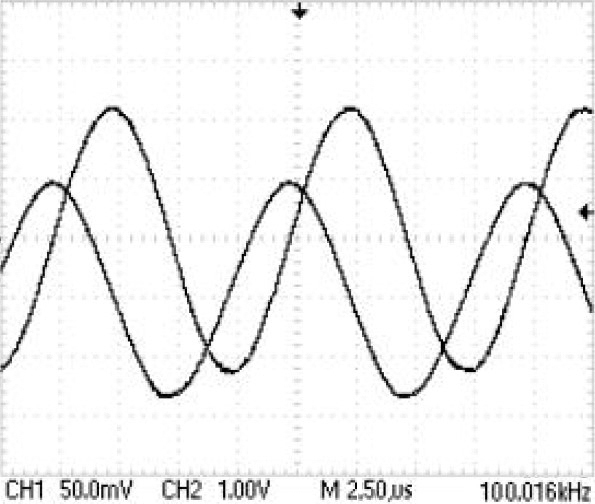
\includegraphics[width=0.85\textwidth]{../oscilloscopio/discriminatore_GBW.jpg}
	\caption{Regime di linearità (alte frequenze e piccolo segnale)}
	\label{fig:GBW}
	\end{minipage}
	\begin{minipage}{0.49\textwidth}
	\centering
	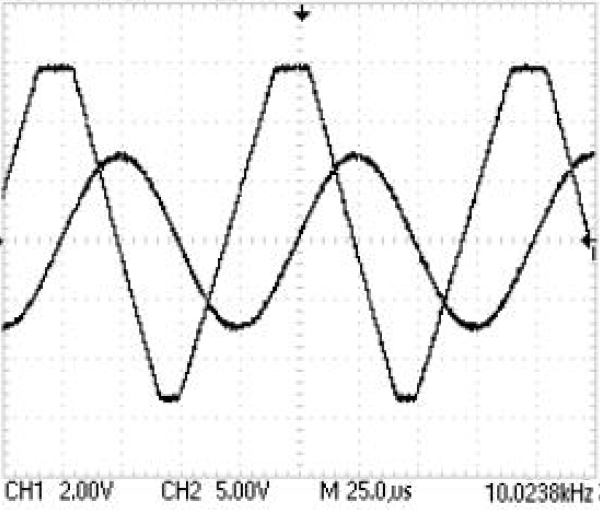
\includegraphics[width=0.85\textwidth]{../oscilloscopio/discriminator_slewrate.jpg}
	\caption{Deformazione dell'onda quadra dovuta allo slew-rate (medie frequenze, grande segnale)}
	\label{fig:slewrate_razzista}
	\end{minipage}
\end{figure}

\subsection{Slew rate}
Per frequenze medio/alte e grandi segnali lo slew-rate produce una notevole distorsione dell'onda quadra limitando la velocità di salita/discesa del segnale. Gli effetti dello slew-rate sulla risposta del circuito sono chiari in \figurename{~\ref{fig:slewrate_razzista}}. Si è misurata la velocità di discesa del segnale, il valore trovato è stato $\unit{13.4 \pm 0.4}{\volt /\micro\second}$, compatibile con il valore di $\unit{13}{\volt / \micro\second}$ riportato nel datasheet.

\section{Amplificatore di carica}

Si è montato il circuito in \figurename{~\ref{circuio_ampli}} con i seguenti valori dei componenti:

\begin{figure}[H]
	\begin{minipage}{0.3\textwidth}
		\centering
		\begin{tabular}{l}
			$C_1 = \unit{21.0 \pm 0.9}{\nano\farad}$  \\ 
			$C_T = \unit{1.00 \pm 0.05}{\nano\farad}$ \\
			$C_F = \unit{1.00 \pm 0.05}{\nano\farad}$ \\
			$R_1 = \unit{99.1 \pm 0.9}{k\ohm}$  \\
			$R_2 = \unit{98.8 \pm 0.9}{\ohm}$
		\end{tabular}
	\end{minipage}
	\begin{minipage}{0.7\textwidth}
		\centering
		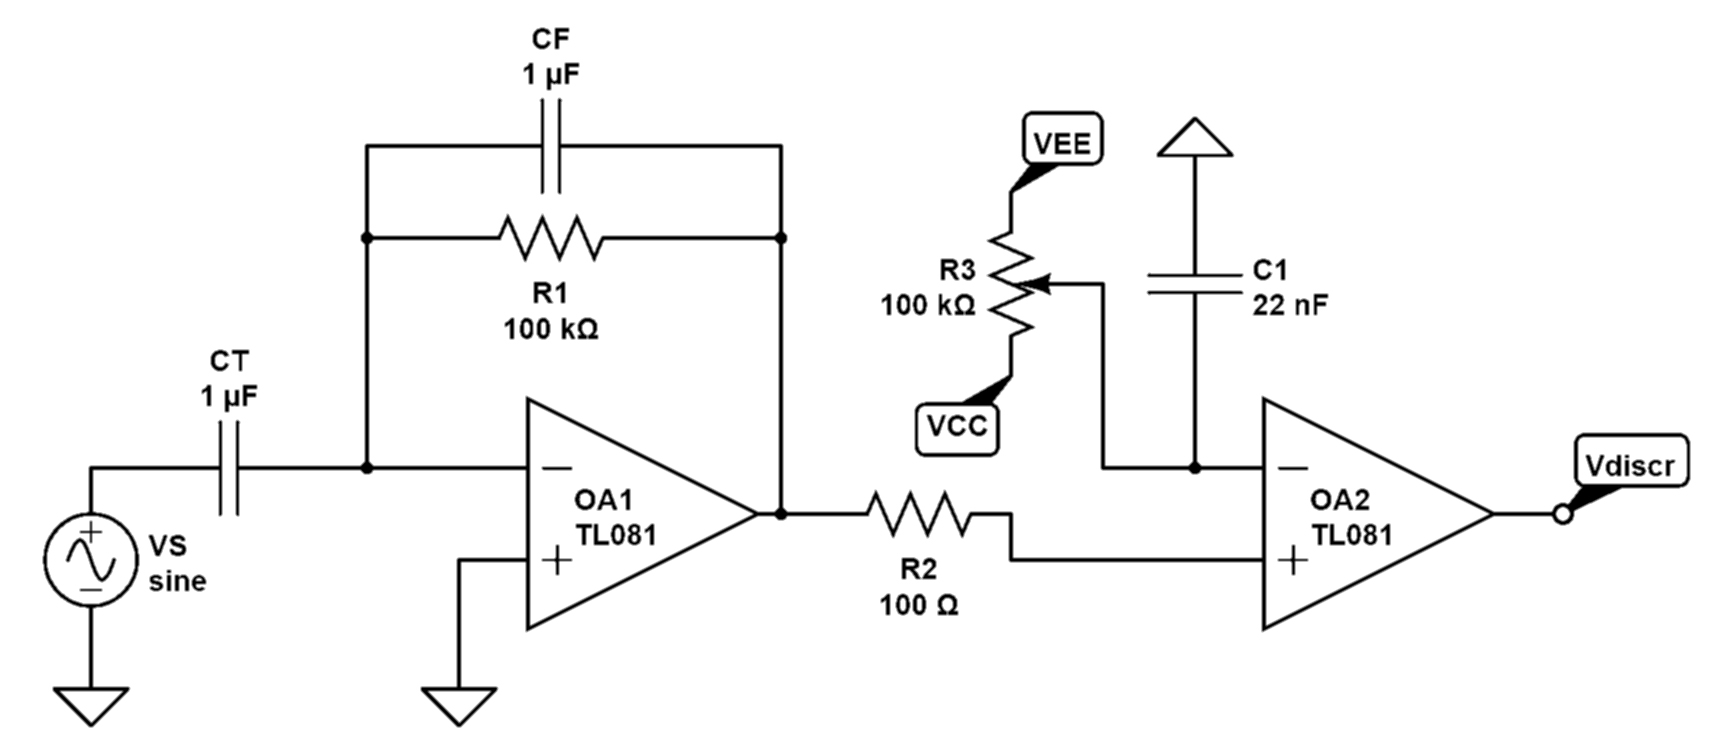
\includegraphics[width=\textwidth]{../circuiti/charge_amplifier.jpg}
		\caption{Schema del circuito amplificatore di carica}
		\label{circuio_ampli}
	\end{minipage}
\end{figure}
 Si è quindi fissato il valore di soglia del discriminatore a $V_0 = \unit{271 \pm 2}{\milli\volt}$.
\subsection{Risposta in condizioni ideali}
Il circuito di iniezione di carica è costituito dal generatore di onde quadre e dal condensatore $C_T$. Il condensatore è messo a terra attraverso l'OpAmp formando quindi un circuito derivatore. Avendo in ingresso un onda quadra il derivatore restituisce degli impulsi che per un generatore di onde quadre ideale sarebbero delle delta, queste vanno a caricare il condensatore $C_F$, la tensione ai cui capi sarà pari alla tensione di alimentazione nell'ipotesi che le capacità $C_F$ e $C_T$ siano uguali.

Il condensatore $C_F$ inizierà quindi a scaricarsi attraverso la resistenza $R_1$ con un tempo caratteristico $\tau = R_1 \cdot C_F$. Quando la tensione sul condensatore scenderà sotto la tensione di soglia fissata attraverso il potenziometro $R_3$, il discriminatore cambierà stato.

L'andamento teorico è stato verificato per una frequenza di $\sim \unit{100}{\hertz}$, che garantisce un'onda quadra ben formata, e un tensione di input di $\unit{6.00 \pm 0.20}{\volt}$, come visibile in \figurename{~\ref{ampli_carica}}. 

La tensione misurata all'inizio della scarica all'output del primo OpAmp è $\unit{5.84 \pm 0.20}{\volt}$, compatibile con quanto atteso e la durata dell'impulso in output è $\unit{312 \pm 2}{\micro\second}$, anch'essa compatibile con il valore atteso $t^{exp} = \tau \cdot \text{ln}(V_{IN}/V_0) = \unit{304 \pm 16}{\micro\second}$.

\subsection{}
Si è misurata la durata del segnale in uscita al variare dell'intensità del segnale in ingresso, i dati raccolti sono riportati in appendice in \tablename{~\ref{tab:V_t}}.
Dalla teoria sappiamo che $t = \tau \cdot \text{ln}(V_{IN}/V_0)$, dove $V_0$ è la tensione di soglia fissata nel discriminatore e $\tau = R_1 \cdot C_F$.

Si sono fittate le misure eseguite, i grafici e i risultati del fit sono di seguito riportanti.

\begin{figure}[H]
	\begin{minipage}{0.28\textwidth}
		\centering
		\begin{tabular}{l}
			$\tau = \unit{99.7 \pm 0.6}{\micro\second}$ \\
			$V_0 = \unit{272 \pm 5}{\milli \volt}$ \\
			$\chi^2 / ndof = 7.8/11$\\
			$corr(\tau,V_0) = -0.956$\\
		\end{tabular}
	\end{minipage}
	\begin{minipage}{0.75\textwidth}
		\centering
		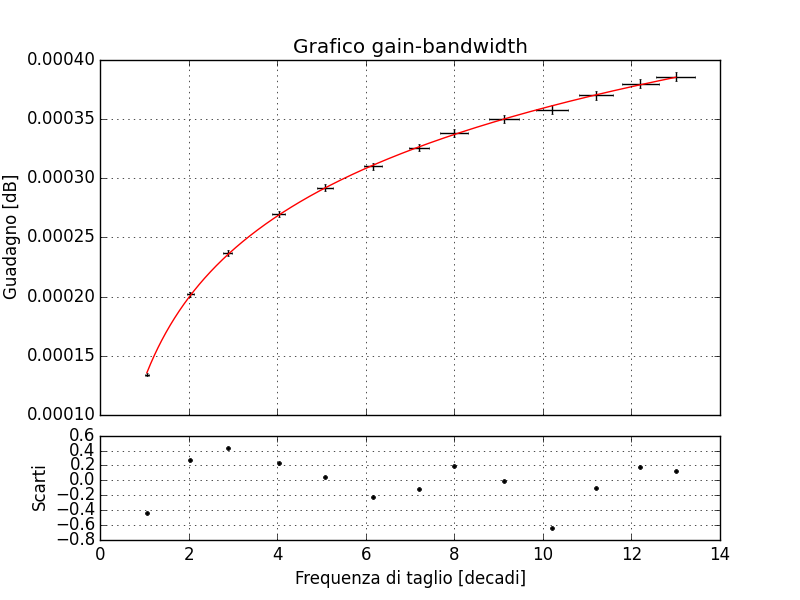
\includegraphics[width=\textwidth]{../grafici/fit_V_t.pdf}
		\caption{Dati e fit sul circuito amplificatore di carica}
		\label{}
	\end{minipage}
\end{figure}

I risultati trovati sono in ottimo accordo con quelli attesi, cioè $\tau^{exp} = \unit{98 \pm 5}{\micro\second}$ e $V_0^{exp} = \unit{271 \pm 2}{\milli\volt}$, la tensione di soglia scelta all'inizio.

Il segnale in uscita è visibile per tensioni di ingresso fino a $V_{lim} = \unit{288 \pm 9}{\milli\volt}$, che come atteso è comparabile con la tensione di soglia fissata, infatti se il segnale in ingresso non supera mai la soglia $V_0$ il discriminatore non cambierà mai stato e non sarà visibile alcun segnale.

Modificando la posizione del potenziometro $R_3$ si modifica la tensione di soglia del discriminatore cambiando di conseguenza la minima tensione in ingresso necessaria ad avere un segnale in output.

\section{Trigger di Schmitt}
Si è montato il circuito in \figurename{~\ref{fig:schmitt_trigger}}.

\begin{figure}[H]
	\centering
	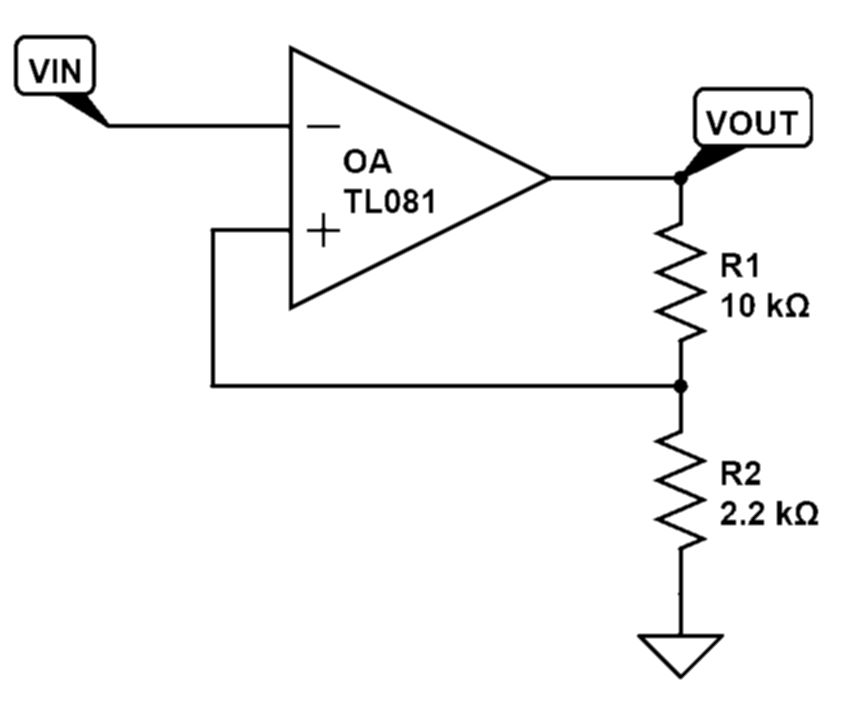
\includegraphics[width=0.40\textwidth]{../circuiti/schmitt_trigger.jpg}
	\caption{Schema del circuito del trigger di Schmitt}
	\label{fig:schmitt_trigger}
\end{figure}

I valori delle resistenze utilizzate sono riportati di seguito:

\begin{table}[H]
	\centering
	\begin{tabular}{cc}
        $ R_1 = \unit{9.88 \pm 0.08}{\kilo\ohm}$  & $R_2 = \unit{2.31 \pm 0.02}{\kilo\ohm}$
	\end{tabular}
\end{table}

Il grafico della risposta ad un segnale sinusoidale è riportato in \figurename{~\ref{fig:schmitt}}.

\begin{figure}[H]
    \centering
    \begin{minipage}{0.49\textwidth}
	    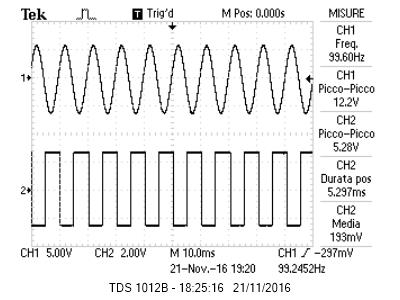
\includegraphics[width=\textwidth]{../oscilloscopio/schmitt.jpg}
	    \caption{Risposta ad un segnale sinusoidale}
	    \label{fig:schmitt}
    \end{minipage}
    \begin{minipage}{0.49\textwidth}
        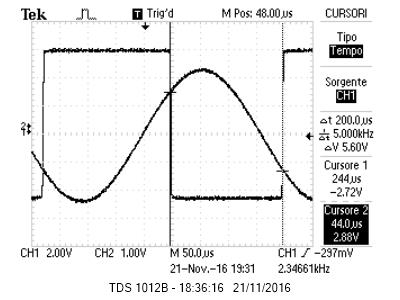
\includegraphics[width=\textwidth]{../oscilloscopio/schmitt_soglia.jpg}
        \caption{Misura delle tensioni di soglia}
        \label{fig:schmitt_soglia}
    \end{minipage}
\end{figure}

Il funzionamento del circuito osservato corrisponde a quanto atteso:
\begin{itemize}
\item il valore di $V_{out}$ è inizialmente fisso ad una delle due tensioni di alimentazione;
\item quando $V_{in}$ supera la corrispondente tensione di soglia $V_{TH}$ scatta, e passa all'altra tensione di alimentazione;
\item quando $V_{in}$ supera la seconda soglia $V_{TL}$ scatta nuovamente, e torna al valore iniziale.
\end{itemize}

I valori delle due soglie sono stati misurati, com'è mostrato in \figurename{~\ref{fig:schmitt_soglia}}, e vengono riportati di seguito:

\begin{table}[H]
	\centering
	\begin{tabular}{cc}
        $ V_{TH} = \unit{2.72 \pm 0.08}{\volt}$  & $V_{TL} = \unit{-2.56 \pm 0.08}{\volt}$
	\end{tabular}
\end{table}

Mentre i valori fra cui oscilla $V_{out}$ sono:

\begin{table}[H]
	\centering
	\begin{tabular}{cc}
        $ V_{H} = \unit{14.0 \pm 0.4}{\volt}$  & $V_{L} = \unit{-13.4 \pm 0.4}{\volt}$
	\end{tabular}
\end{table}

I valori attesi per le tensioni di soglia sono $V_{TH}^{exp} = V_H \cdot R_2/(R_1+R_2) = \unit{2.65 \pm 0.09}{\volt}$ e $V_{TL}^{exp} = \unit{2.54 \pm 0.08}{\volt}$, entrambe in accordo con le misure effettuate. 
 

\subsection{Risposta in ampiezza} Se si aumenta l'ampiezza del segnale in ingresso il funzionamento del circuito rimane qualitativamente lo stesso: per tensioni d'ingresso al di fuori dell'intervallo definito dalle due soglie il valore dell'uscita rimane costante. Per segnali di ampiezza sufficientemente bassa invece non si riesce a superare i valori di soglia, e l'uscita rimane fissa su una delle due tensioni di alimentazione.

\subsection{Risposta in frequenza} A bassa frequenza il circuito riproduce il comportamento ideale precedentemente descritto. Ad alta frequenza l'output è invece limitato dallo slew rate nelle transizioni tra i due stati, perciò quella che nel caso ideale dovrebbe essere un'onda quadra viene deformata, come risulta in \figurename{~\ref{fig:slew_rate}}, riprodotta di seguito.

Si nota che, come riportato da datasheet, lo slew rate in salita e in discesa non coincide, in particolare il primo è inferiore al secondo, con valori rispettivamente di $\unit{11.4 \pm 0.4}{\volt/\micro\second}$ e $\unit{13.0 \pm 0.4}{\volt/\micro\second}$, misurati ad una frequenza di $\unit{138 \pm 1}{\kilo\hertz}$.

\begin{figure}[H]
	\centering
	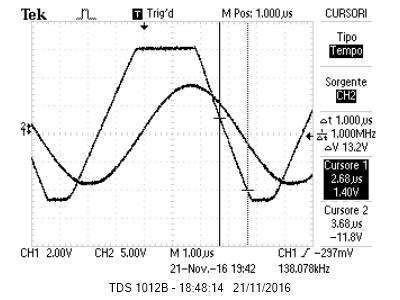
\includegraphics[width=0.40\textwidth]{../oscilloscopio/schmitt_slewrate.jpg}
	\caption{Effetto dello slew rate dell'OpAmp sull'output}
	\label{fig:slew_rate}
\end{figure}

Si ha perciò che il comportamento del circuito è ideale per frequenze tali per cui lo slew rate non porta ad un tempo di \emph{switching} comparabile al semiperiodo dell'onda quadra. Perciò, dato il valore dello slew rate in salita, si può affermare che il circuito abbia un comportamento ideale per frequenze fino a $\sim \unit{6}{\kilo\hertz}$, per cui il tempo di \emph{switching} è $\sim 1\%$ del semiperiodo.

% Problema: come diamine si giustifica la discesa più rapida dello slew_rate? Io ce la scriverei, ma due righe di ipotesi andrebbero scritte.

\section{Multivibratore astabile}
Si è montato il circuito del multivibratore astabile in \figurename{~\ref{fig:multivibratore}}.

\begin{figure}[H]
	\centering
	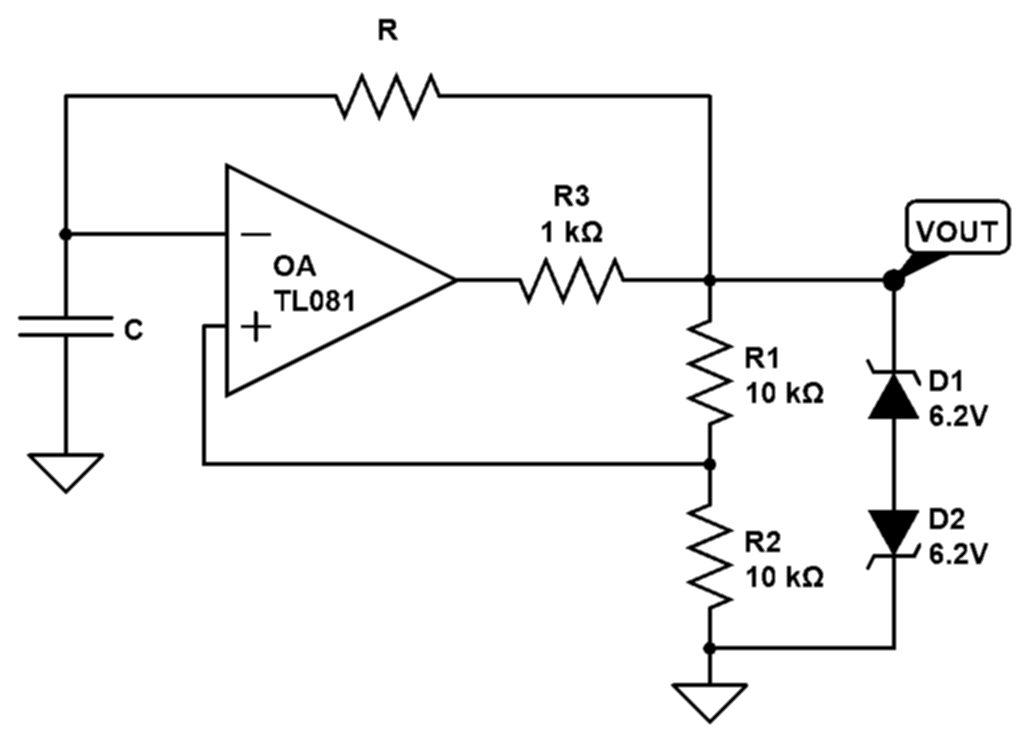
\includegraphics[width=0.40\textwidth]{../circuiti/multivibratore.jpg}
	\caption{Schema del circuito del multivibratore astabile}
	\label{fig:multivibratore}
\end{figure}

Come ricavato a lezione il periodo di oscillazione dell'output è pari a 
\begin{equation}
\label{periodo}
T = 2 \tau \text{ln}(1 + 2 R_2/R_1)
\end{equation}
ed è indipendente dalla tensione di breakdown degli Zener $V_Z$.

Si sono scelti di conseguenza dei valori di $R$ e $C$ tali che il periodo fosse $\sim \unit{2}{\milli\second}$ come richiesto. I valori misurati, di questi e degli altri componenti, sono riportati di seguito.

\emph{Si è scelto $C$ in modo che sia piuttosto grande rispetto alle capacità parassite della basetta, che sono attese dell'ordine delle decine di pF}

\begin{table}[H]
	\centering
	\begin{tabular}{ccccc}
        $ R_1 = \unit{9.88 \pm 0.08}{\kilo\ohm}$ & $R_2 = \unit{9.88 \pm 0.08}{\kilo\ohm}$ & $R_3 = \unit{983 \pm 8}{\ohm}$ & $R = \unit{8.13 \pm 0.07}{\kilo\ohm}$ & $C = \unit{109 \pm 4}{\nano\farad}$
	\end{tabular}
\end{table}

\subsection{Analisi del funzionamento}
L'OpAmp amplifica qualunque minima differenza di tensione fra i due terminali di input, si avrà quindi che, non pilotando gli ingressi con alcuna tensione di input, qualche minima differenza di tensione, dovuta quindi al rumore, venga amplificata (è molto facile che già questo porti l'output a saturazione).

Si viene dunque a creare una differenza di potenziale ai capi della resistenza $R$ che induce una corrente e porta infine alla carica del condensatore $C$.

Il condensatore $C$, caricandosi, porterà a un certo punto la tensione al terminale '-' a oltrepassare, in positivo o in negativo a seconda dello stato di $V_{out}$, la tensione al terminale '+', necessariamente minore in modulo di $V_{out}$ in quanto determinata dal partitore $R_1 - R_2$.

Non appena avviene questo passaggio lo stato dell'ouput salta, e satura all'altro stato, determinando quindi un'inversione della corrente che scorre attraverso la resistenza $R$ e invertendo la carica del condensatore.

Raggiunta nuovamente la soglia determinata da $V_+$ l'output scatta di nuovo e cambia stato, e così via. Il tempo con cui avviene questo processo è quello riportato sopra nella formula per il periodo, ed è fissato dal tempo impiegato dal processo di carica del condensatore per raggiungere la soglia fissata da $V_+$, quindi come atteso dipenderà solamente dalla costante $\tau$ del circuito $R-C$ e dal rapporto di partizione del partitore $R_1-R_2$.

\subsection{Analisi dei segnali in ingresso e in uscita dall'OpAmp}
I segnali $V_+$, $V_-$ e $V_{out}$ sono rappresentati nelle figure~\ref{fig:multivibratore-} e \ref{fig:multivibratore+}, in particolare:
\begin{description}
\item[\figurename{~\ref{fig:multivibratore-}}] sono raffigurati i segnali $V_-$ e $V_{out}$, rispettivamente la \emph{pinna di squalo} e l'onda quadra;
\item[\figurename{~\ref{fig:multivibratore+}}] sono raffigurati i segnali $V_+$ e $V_{out}$, entrambi onde quadre, ma il primo è minore in modulo del secondo in entrambi gli stati a causa del partitore $R_1-R_2$.
\end{description}

\begin{figure}[H]
    \centering
    \begin{minipage}{0.49\textwidth}
        \centering
        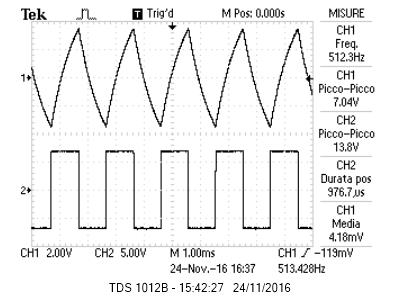
\includegraphics[width = \textwidth]{../oscilloscopio/multivibratore.jpg}
        \caption{Tensioni di output e al terminale '-' nel multivibratore}
        \label{fig:multivibratore-}
    \end{minipage}
    \begin{minipage}{0.49\textwidth}
        \centering
        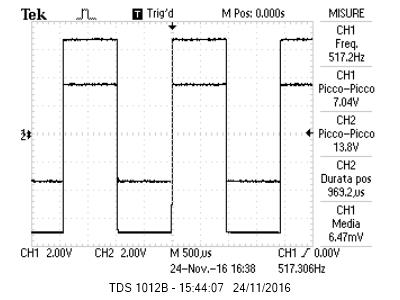
\includegraphics[width = \textwidth]{../oscilloscopio/multivibratore_V+.jpg}
        \caption{Tensioni di output e al terminale '+' nel multivibratore}
        \label{fig:multivibratore+}
    \end{minipage}
\end{figure}

\paragraph{Tensione $V_{out}$} I valori misurati per gli stati alto e basso dell'output e di $V_+$ sono:

\begin{table}[H]
	\centering
	\begin{tabular}{cc}
        $ V_{out H} = \unit{6.9 \pm 0.2}{\volt}$  & $V_{out L} = \unit{-6.9 \pm 0.2}{\volt}$\\
        $ V_{+ H} = \unit{3.52 \pm 0.11}{\volt}$  & $V_{+ L} = \unit{-3.52 \pm 0.11}{\volt}$
	\end{tabular}
\end{table}

Che è consistente con quanto atteso. Infatti gli Zener hanno una tensione di breakdown pari a $\sim \unit{6.2}{\volt}$, aggiungendo $V_\gamma$ (cioè la tensione a cui il diodo passa in conduzione, o forward voltage), che da datasheet è al più $\unit{1.5}{\volt}$, si ha effettivamente la consistenza del valore misurato.

\paragraph{Zener e $R_3$} Quello che succede è che la tensione al terminale di output dell'OpAmp, dovuta all'alimentazione, è maggiore della massima caduta di tensione fissata dagli Zener. Per questo ai capi della resistenza $R_3$ si ha una data caduta di potenziale (che corrisponde a $V_{CC}-V_Z$), che porta ad una corrente che fluisce nella resistenza. In questo modo è possibile fissare il valore dei due stati di $V_{out}$ coi soli Zener, rendendo tali valori indipendenti dal valore dell'amplificazione dell'OpAmp e dall'alimentazione.

\paragraph{Tensione $V_+$} Riguardo $V_+$ si ha che questa è determinato da $V_{out}$ e dal rapporto di partizione $R_1 - R_2$, che in questo caso, poiché $R_1 \sim R_2$ è circa la metà. Per l'esattezza il rapporto di partizione atteso è pari a $V_Z R_2/(R_1 + R_2) = \unit{0.5000 \pm 0.0028}$ mentre il rapporto fra le due tensioni misurate è pari a $\unit{0.510 \pm 0.022}$, e quindi i due valori sono compatibili.

\paragraph{Tensione $V_-$} Questo segnale, come già detto e come si può osservare dalla \figurename{~\ref{fig:multivibratore-}, è una tipica onda a \emph{pinna di squalo}, cioè la successione di esponenziali crescenti e decrescenti, dovuti alle cariche e scariche del condensatore $C$. I valori misurati per le tensioni nei punti d'inversione sono $\pm \unit{3.52 \pm 0.11}{\volt}$.
	
La tensione nei punti di inversione è dunque esattamente la stessa che si ha per $V_+$, come atteso dato l'altissimo valore di amplificazione dell'OpAmp.

\paragraph{Periodo del segnale} La frequenza del segnale, determinata dalla legge \eqref{periodo}, è pari a $\unit{510 \pm 40}{\hertz}$, mentre quella misurata è $\unit{513 \pm 5}{\hertz}$, perciò evidentemente compatibili.

\subsection{Dipendenza del periodo di $V_{out}$ dalla tensione di alimentazione}
Ci si aspetta che il periodo sia indipendente dalla tensione di alimentazione, fintanto che questa mantenga un'uscita al di sopra della tensione di breakdown degli Zener (in realtà breakdown più la tensione di conduzione, cioè quei $\sim \unit{6.9}{\volt}$ misurati precedentemente).
Al di sotto di questa tensione non è più fissato il valore di $V_{out}$, e di conseguenza neanche i valori delle soglie (cioè $V_+$), che determinano infine il tempo di crescita dell'esponenziale, dovuto alla carica del condensatore $C$.

Per questo, quando si diminuisce il valore della tensione di alimentazione diminuisce il periodo, o meglio la durata della semionda. Si può infatti diminuire anche una sola delle due tensioni di alimentazione, ottenendo così un segnale in output sempre a due stati, ma due stati con tensioni diverse anche in modulo, e soprattutto di durata differente; in sostanza si arriva a cambiare sia la media che il duty cycle del treno d'impulsi, in modo non indipendente.

Si riporta in \figurename{~\ref{fig:fig1}} e \figurename{~\ref{fig:fig2}} due esempi di quanto descritto, il primo con una tensione sopra il livello degli Zener e il secondo sotto tale livello, entrambi però con alimentazioni approsimativamente simmetriche.

\begin{figure}[H]
    \centering
    \begin{minipage}{0.49\textwidth}
        \centering
        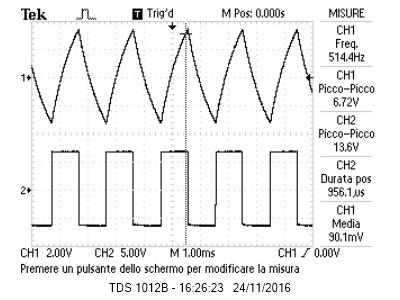
\includegraphics[width = \textwidth]{../oscilloscopio/fig1.jpg}
        \caption{Segnale in uscita modulato dai diodi Zener}
        \label{fig:fig1}
    \end{minipage}
    \begin{minipage}{0.49\textwidth}
        \centering
        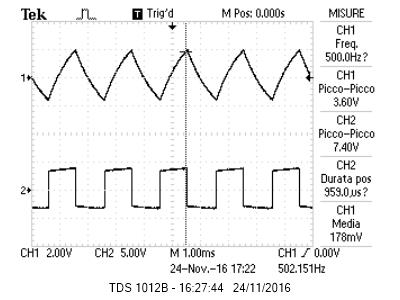
\includegraphics[width = \textwidth]{../oscilloscopio/fig2.jpg}
        \caption{Segnale in uscita modulato dalle tensioni di alimentazione dell'OpAmp}
        \label{fig:fig2}
    \end{minipage}
\end{figure}

\subsection{Limiti in frequenza dell'onda quadra generata}
Si è provato a sostituire il condensatore $C$ e la resistenza $R$ in modo da aumentare la frequenza dell'oscillazione. Per frequenze troppo alte si ha che il segnale in uscita approssima sempre peggio un'onda quadra, fino ad essere molto deformato (si veda \figurename{~\ref{fig:scazzo}}).

\begin{figure}[H]
        \centering
        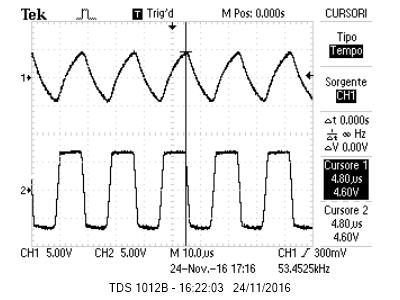
\includegraphics[width = 0.49\textwidth]{../oscilloscopio/multivibratore_scazzo.jpg}
        \caption{Multivibratore oscillante ad una frequenza di $\sim \unit{53}{\kilo\hertz}$}
        \label{fig:scazzo}
\end{figure}

Si è trovato che il circuito approssimativamente genera in output un'onda quadra fino alla frequenza di $\sim \unit{10}{\kilo\hertz}$.

\pagebreak
\section{Appendice: Dati acquisiti}
Si riportano qui le tabelle dei dati usati per i fit e i grafici.

\centering
\begin{figure}[h!]
	\begin{minipage}[t]{0.49\textwidth}
		\centering
		\resizebox{0.7\textwidth}{!}{
		\input{../tabelle/tab_gain_bandwidth.txt}}
		\captionof{table}{Conservazione GBW}
		\label{tab:GBW}
	\end{minipage}
	\begin{minipage}[t]{0.5\textwidth}
		\centering
		\resizebox{0.7\textwidth}{!}{
		\input{../tabelle/tab_V_t.txt}}
		\captionof{table}{Tensione input vs TOT}
		\label{tab:V_t}
	\end{minipage}
\end{figure}




\end{document}
